\subsubsection{PatternMaker}
Upon realizing this theoretical maximum, we began to approach the problem differently: rather than problem mimicking biological behavior, this became a packing problem, or an environment that had to be most efficiently utilized.  Rather than attempting to hardcode behaviors into the organisms, we gave each one of six specific roles.  These role were differentiated on two counts:
\begin{enumerate}
\item Each role only reproduced children of one or two other specific roles in a specific direction, and
\item Each role only ��harvested�� the farm at a specific, unique point during a 32-turn cycle.
\end{enumerate}

Each organism had a cyclical concept of a turn number which was incremented every turn.  This, rather than energy thresholds, determined when behaviors would happen.  PatternMaker organisms on their own are very dumb, but collectively, they do an excellent job of maximising the resources on the board.

\begin{figure}[htf]
\centering
  % Requires \usepackage{graphicx}
  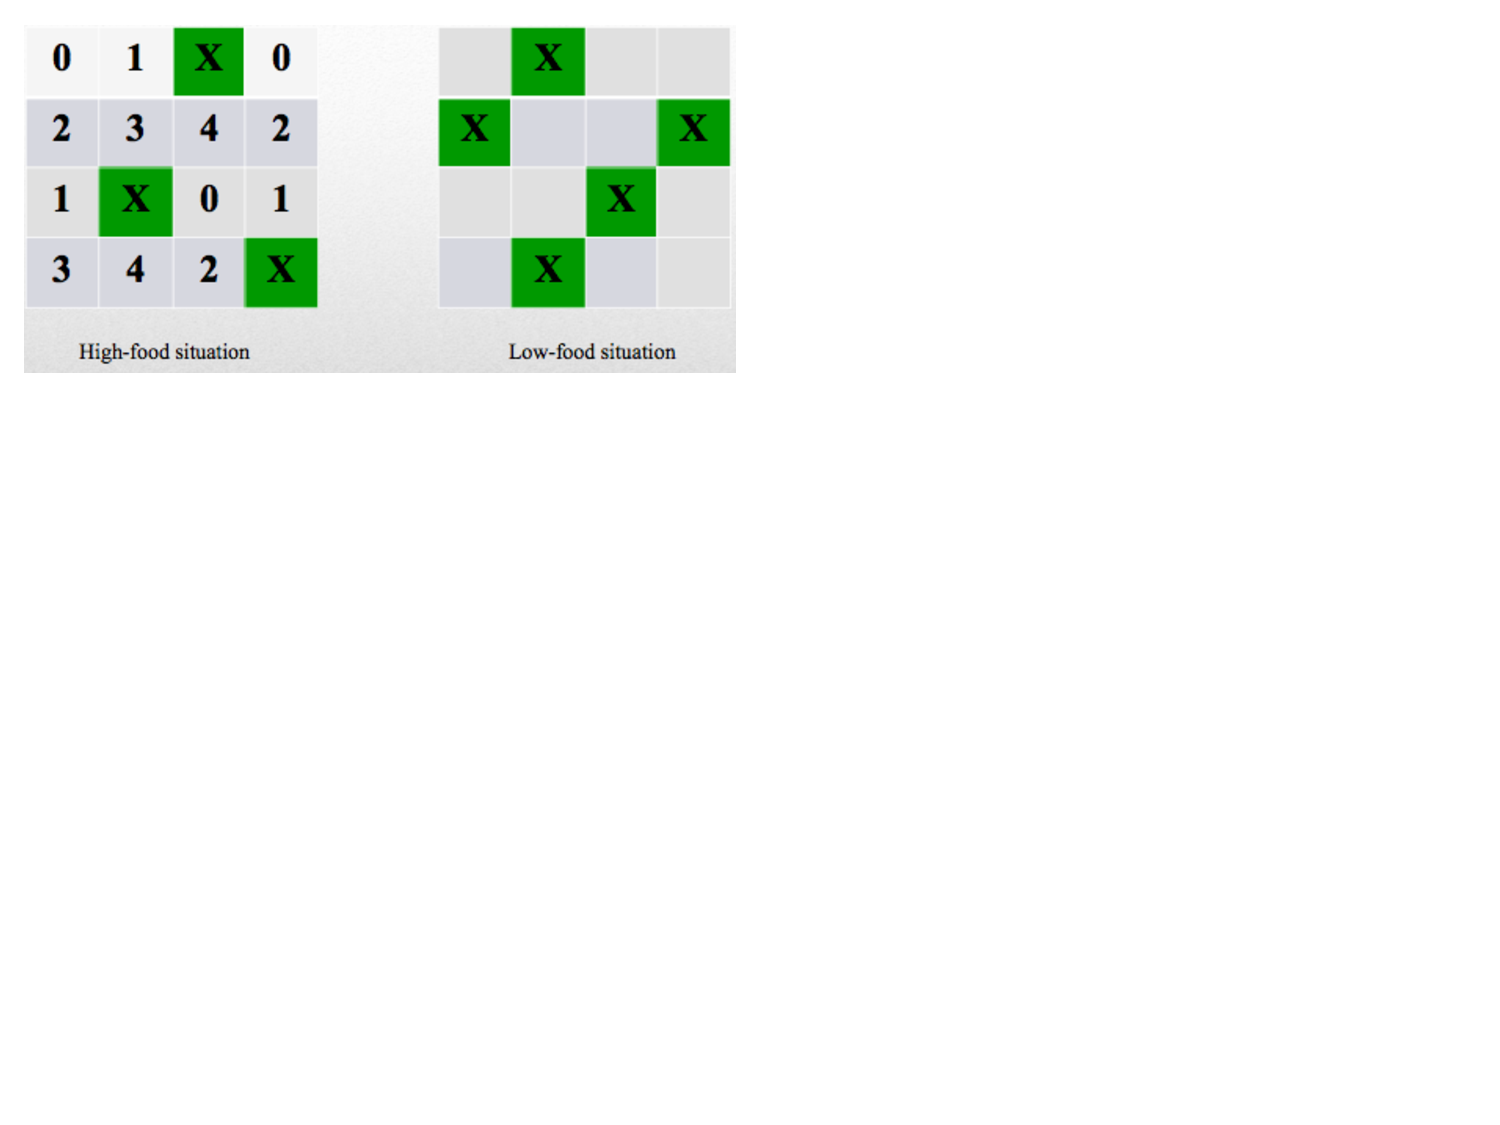
\includegraphics[trim=10mm 130mm 135mm 10mm]{figs/high-low-food.pdf}\\
  \caption{PatternMaker harvesting patterns in high- and low- food situations}
  \label{fig:high-low-food}
\end{figure}


Another PatternMaker organism was developed to deal with low-food situations.  This patternmaker relied on the same concept described above, but instead allowed each organism to be orthogonal to two farms instead of one.  This resulted in separated, diagonal patterns rather than L-shaped ones (see Figure~\ref{fig:high-low-food}).

An attempt was made to reconcile the Talker and PatternMaker strategies.  The goal was to identify whether the board has a high or low q value and then generate the corresponding pattern.  However, this proved to be ineffective: even after identifying a data-robustness level sufficient to make a patterning decision, patterning proved ineffective because of the residual Talker organisms left on the board. 